\documentclass[11pt]{article}
\usepackage{royden-report}
\newcommand{\topic}[1]{\par\smallskip\noindent\textbf{#1}\quad}
\setlength{\textfloatsep}{10pt}
\renewcommand{\arraystretch}{1.17}
\makeatletter
\long\def\@makecaption#1#2{\vskip6pt{\small #1: #2\par}}
\makeatother
\hypersetup{pdftitle={The Dysthe Project: A Plain-Language Progress Report}}
\begin{document}
\begin{center}
{\Large The Dysthe Project}\\[5pt]
A plain-language progress report\\[6pt]
Work reviewed through 23 September 2026
\end{center}

\section*{1. What is this project trying to do?}
The project asks how a concentrated group of waves changes as it travels.
Does it spread out? Keep its shape? Break into smaller features? What
happens when two groups meet? A second question has become increasingly
important: can artificial intelligence learn to predict these changes
without repeating the full calculation every time?

A model is a simplified set of rules for how a system behaves.
A useful picture is a short burst of light rather than an endless, steady
beam. The burst contains many fast oscillations. Instead of tracking every
one, a wave model can describe the overall shape surrounding them. That
shape is called the \emph{envelope}, much as the outline of a musical sound
shows when it grows louder and fades.

Dysthe equations describe certain kinds of wave-envelope behavior. The
project began with these models and has since branched into plasma, a state
of matter containing free electrically charged particles. The connection is the approach
to computing and learning physical behavior. The plasma experiment uses
its own equations for particle motion and electric fields.

\topic{Where the work stands}
There are now working simulation programs, a collection of checked
experiments, two approaches to AI prediction, and tools for running and
reviewing large computer jobs. One early AI model matched a short light-wave
test closely. The more general plasma model still makes substantial
physical errors. The work has therefore produced both useful capabilities
and a much clearer picture of what needs improving.

\begin{center}
\small
\begin{tabular}{@{}p{3.1cm}p{6.2cm}p{5.9cm}@{}}
\toprule
Part of the project & What it studies & What to keep in mind \\
\midrule
Light-wave models & How a pulse spreads, concentrates or changes shape. & The main study of light-pulse evolution. \\
Water-wave model & Traveling pulses and collisions in a simpler setting. & A separate equation and a separate test. \\
Plasma extension & Electron motion and the electric field it creates. & A new test of AI prediction, using different physics. \\
\bottomrule
\end{tabular}
\end{center}

\topic{How to read this report}
Pages 2--3 explain the wave simulations. Page 4 introduces the AI work.
Page 5 explains the latest plasma results. Page 6 describes the practical
outcome and next steps. There are no equations to learn. Every numerical
result is from a computer experiment, not a laboratory measurement.

\clearpage
\section*{2. First, understand how waves spread}
The first calculations used a simplified setting called a \emph{linear}
model. Here, small component waves evolve independently and can be added
together. This makes it easier to understand what the computer should do
before introducing interactions that are harder to predict.

The main tool was \emph{Fourier analysis}: separating a complicated wave
into simpler repeating patterns. It is similar to identifying individual
notes in a chord. The program advances each component and combines them
again to recover the evolving pulse.

\topic{What was built}
A simulator that accepts different starting shapes and tracks their
strength, width and movement. The experiments varied the starting pattern,
the direction of its oscillations and the model's physical settings.
Plots, three-dimensional views and animations made the movement easier to
inspect. Separate mathematical tests examined how quickly selected measures
of wave strength fall as a pulse spreads.

\begin{figure}[h!]
\centering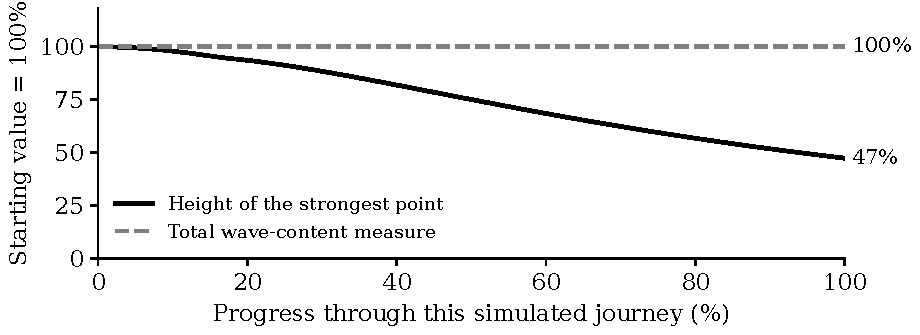
\includegraphics[width=.95\linewidth]{figures/spreading.pdf}
\caption{One computed light-wave example. The strongest point drops to
about 47\% of its starting value while the total wave-content measure stays
constant. Both lines are scaled to their own starting values. This is
spreading, not evidence that the missing peak strength became heat.}
\end{figure}

\topic{What was learned}
A lower peak does not mean that the whole wave has disappeared. The same
wave content can occupy a wider region, with a smaller highest point.
Different starting oscillations can also produce different spreading,
even when the initial outlines look identical.

Longer simulations exposed a practical problem: the strongest part of a
wave can move far outside the area originally being watched. The project
therefore enlarged its search region, increased numerical detail, and
compared selected answers with an independent calculation. Four demanding
late-time examples passed the chosen checks on their peak values. Additional
frequency and specially chosen input tests explored which patterns deserve
closer mathematical attention.

\topic{What this does not establish}
These experiments support particular computed examples. They do not prove
a rule for every possible wave or for indefinitely long travel. Some earlier
results changed when the computational region was enlarged; those needed
refinement before interpretation. The plots are evidence to investigate,
not a replacement for a mathematical proof.\,[1]

\clearpage
\section*{3. Then, let waves influence their own motion}
In a \emph{nonlinear} model, the strength of a wave changes how it evolves.
A familiar analogy is traffic: a few cars move almost independently, but
a crowded road changes how every driver can move. For waves, these
interactions can compete with spreading and sometimes help a pulse keep
its shape.

\topic{Traveling pulses and collisions}
The project built a nonlinear simulator and checked it against a simpler
case with a known mathematical answer. It then computed 28 traveling-pulse
shapes for the water-wave model and tested their motion, small disturbances
and collisions.

The collision tests showed that the outgoing pulses did not perfectly
recover their original shapes. About 1.8\% of the measured wave content
appeared outside the two chosen main-pulse regions, beyond what was there
initially. That number depends on how the regions are drawn; it is evidence
of a small leftover disturbance, not a claim that energy vanished.\,[2]

\begin{figure}[h!]
\centering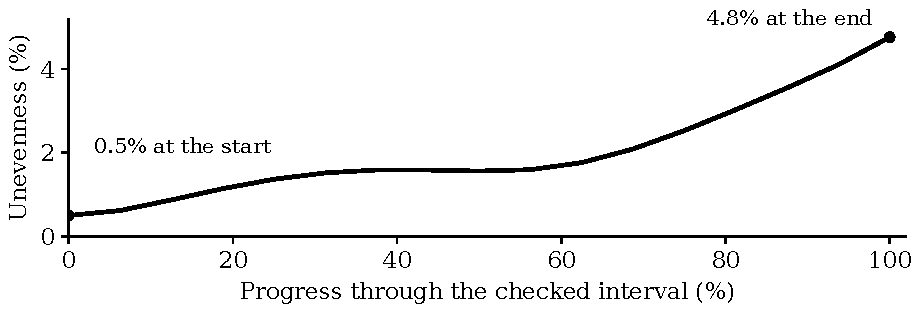
\includegraphics[width=.95\linewidth]{figures/unevenness.pdf}
\caption{A different experiment, using the light-wave model: a small
variation across a stripe-shaped pulse grew from about 0.5\% to 4.8\%.
This measures unevenness in the wave pattern, not a percentage increase in
its peak height. Only the interval supported by checks using finer calculations is shown.}
\end{figure}

\topic{Small disturbances can matter}
The optical experiment shows that a deliberately introduced unevenness can
grow. Finer calculations supported the early growth. Later images changed
substantially when the numerical detail changed, so they cannot yet establish
whether the pulse eventually breaks apart or collapses. Nor do these
stripe-shaped examples establish an isolated, stable three-dimensional pulse.

\topic{Looking much farther ahead}
Separate long optical runs showed repeated tightening and loosening that
looked like ``breathing.'' These simulations used a repeating box: a wave
leaving one side reappears on the opposite side, like a character wrapping
around the edge of a video game. Such a box can affect long-term behavior.
One coarse preview also stopped after a consistency check failed. The
observations are therefore clues to investigate, not proof of a permanently
breathing pulse in open space. These long runs were conventional simulations,
not successful long-term AI forecasts.\,[3]

\clearpage
\section*{4. Can AI learn a useful shortcut?}
A conventional simulator repeatedly applies the model's rules. An AI model
instead learns an adjustable approximation. The hope is to obtain useful
predictions quickly after training. That speed advantage must still be
measured at an acceptable level of accuracy; it has not been established
for the current plasma predictor.

\topic{The first approach: learn one chosen problem}
A physics-informed neural network, or \emph{PINN}, was trained to follow
the optical equation. The equation acts like a set of rules for marking
its answers. The starting pulse was built into the model.

After 20,000 training updates, a run on a research computer had a largest
overall wave-pattern mismatch of about \textbf{0.67\%} over its short test interval. The
comparison checked both the strength and oscillation information in the
wave. Separate tests supported the numerical reference on that fixed box.
This is a useful result for one prescribed starting pulse, not evidence
that the network can handle any pulse or predict indefinitely. Changing
the starting condition requires retraining this implementation.\,[3]

\topic{The next approach: learn a family of problems}
A Fourier neural operator, or \emph{FNO}, takes a whole field as input and
predicts its next state. A field is simply a map giving a value at every
location, like a temperature map. The goal is to learn from many examples
and then handle new starting states within the tested range. It reuses
Fourier ideas to recognize patterns at different spatial scales.\,[4]

\begin{figure}[h!]
\centering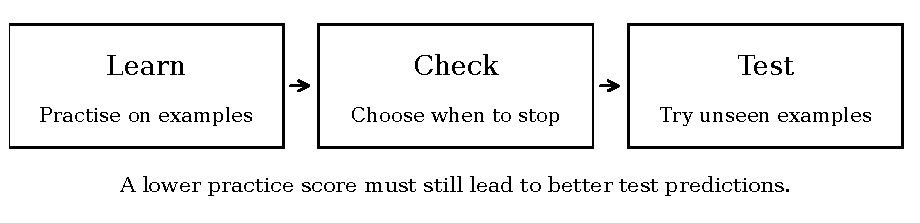
\includegraphics[width=\linewidth]{figures/learning.pdf}
\caption{The learning process separates examples used for practice,
examples used to choose a model, and examples reserved for its final test.
The final test loses that independence if it is repeatedly used to tune the model.}
\end{figure}

\topic{Why more training is not always better}
The early plasma campaign improved on its practice examples while its
longer, self-generated predictions became worse. Feeding each prediction
back into the model lets small mistakes accumulate. A good practice score
therefore did not guarantee a good forecast.

The follow-up added \emph{early stopping}: stop when the separate checking
examples stop improving, and retain the best saved model. It also tested
longer prediction sequences during training and added penalties for
violating physical rules, such as creating or losing particles or energy.
Training logs now show the separate errors,
stopping reason and resource use. These changes make mistakes easier to
find; they do not automatically make the predictions correct.

\clearpage
\section*{5. What did the plasma experiments show?}
Plasma contains charged particles whose motion and electric fields affect
one another. This project uses a deliberately simplified model: electrons
move along one direction while a background of positive charge stays fixed.
Rather than tracking every electron, it predicts a map of how many electrons
are at each location and moving at each speed.

One test concerns \emph{Landau damping}: a collective electric oscillation
weakens as energy transfers into particle motion. Predicting that behavior
requires getting the evolving pattern right, not just making a curve go down.
The study does not include magnetic fields, collisions or a laboratory
plasma experiment.\,[4]

\topic{First campaign: a working model with serious weaknesses}
Three independently initialized training runs performed better than simply
assuming nothing would change. But their particle-motion patterns and
energy bookkeeping could be badly wrong, even when the electric-field
average looked promising. The best saved models occurred well before the
training ended. This motivated the stopping rules and physics checks in
the follow-up.\,[5]

\topic{Latest campaign: the tradeoff became clearer}
The follow-up completed 15 training runs across five setups, then tested the
selected setup and a comparison setup in six evaluations. It reserved 44
fresh random cases and four named checks. Total recorded time was about
10.5 hours on one graphics processor.

\begin{figure}[h!]
\centering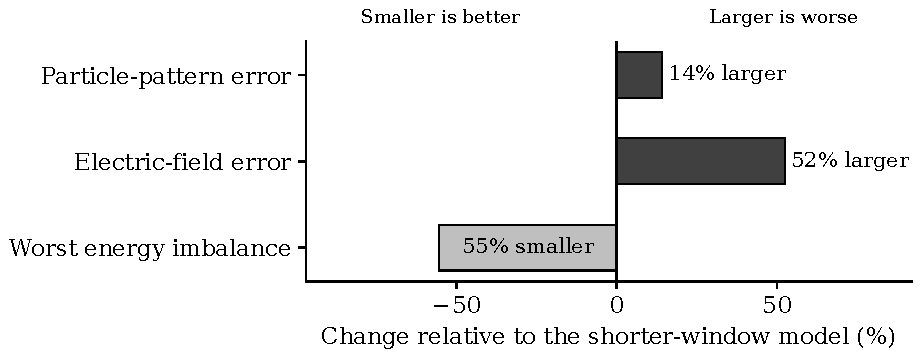
\includegraphics[width=\linewidth]{figures/tradeoff.pdf}
\caption{Within the latest campaign, the selected model was trained on
longer sequences. It reduced its worst energy imbalance but made larger
average particle-pattern and electric-field errors. These are changes in
error measures, not percentages of an answer that is ``correct.''}
\end{figure}

Its worst energy imbalance fell from about 31\% to 14\%, still above the
study's 5\% limit. Every evaluated model failed seven of eight acceptance
checks. The selected model's combined checking score had hidden an important
tradeoff: improving one physical measure made other predictions worse.
A drawing can use the right amount of ink and still show the wrong picture.

The version with an extra penalty for breaking the evolution equation
improved that particular checking measure, but reached its time limit while
still improving. It was not selected for final testing, so its full potential
remains unresolved. The two campaigns also used different test sets and
training budgets; their headline percentages are not a controlled
before-and-after ranking.\,[6]

\clearpage
\section*{6. What has the project accomplished?}
The project has produced a reusable way to investigate wave behavior:
write down a particular physical model, compute examples, check the answers,
and test whether an AI approximation can reproduce them. The main value is
both the software and the evidence about where it can and cannot be trusted.

\topic{The practical work behind the results}
There are now simulation programs for several clearly identified models;
checks against known answers and finer calculations; measures of peaks,
spreading, shape and physical consistency; and saved results, animations and
editable reports. Cluster-job scripts handle larger calculations, training
checkpoints allow work to resume, and export tools bring results back for
review. The latest reports keep small numerical datasets alongside sharp,
zoomable figures so the evidence can be inspected again.

\topic{What remains open}
The work has not demonstrated a universal law for long-term wave decay, a
stable isolated three-dimensional pulse, or a broadly reliable plasma AI.
The short optical AI result is encouraging within its limited test. The
plasma results show why a model must pass several checks at once. None of
these studies has yet been validated against laboratory measurements.

\topic{The next useful step}
Improve plasma predictions over short periods before asking for
much longer forecasts. Keep pattern accuracy and conservation checks separate
when choosing a model. Give the physics-based training a fair comparison,
retain enough output to diagnose failures, and use a new final test set
once the present results have guided changes. For the wave simulations,
longer runs still need checks that distinguish real structure from the
repeating box and numerical error.

\begin{center}
\small
\begin{tabular}{@{}p{3cm}p{12.1cm}@{}}
\toprule
Useful word & Plain-language meaning \\
\midrule
Simulation & A computer calculation of a specified physical model. \\
Reference & A carefully checked calculation used for comparison, not an infallible answer. \\
Training step & One adjustment to an AI model; not a moment of physical time. \\
Conservation & Keeping quantities that the model says should stay constant, such as total energy. \\
Norm & A numerical ruler for measuring a whole pattern; different rulers emphasize different features. \\
Validation & Separate checking examples used during model development. \\
\bottomrule
\end{tabular}
\end{center}

\smallskip
\noindent\textbf{Where the evidence comes from}\par
{\small\raggedright
[1] Project wave-spreading reports, saved histories and spatial-reliability checks,
including the September 10 checkpoint.\\[3pt]
[2] \emph{Nonlinear Solitary-Wave Report}, September 14, and its saved results.
The water-wave model follows \href{https://arxiv.org/abs/1110.4083}{Fedele and Dutykh's spatial Dysthe study}.\\[3pt]
[3] Optical PINN evaluation \texttt{evaluation-001}, its separate reference audit,
and \emph{Technical Review of the Late-Time Experiment}, September 18.\\[3pt]
[4] Background: \href{https://www.energy.gov/science/doe-explainsplasma}{US Department of Energy, plasma};
\href{https://arxiv.org/abs/2010.08895}{Li et al., Fourier neural operators};
\href{https://arxiv.org/abs/1407.1932}{Parker and Dellar, kinetic plasma simulation}.\\[3pt]
[5] Review of overnight plasma job 77761, September 21.\\[3pt]
[6] \href{https://github.com/matasvai/dysthe-pinn/blob/b9630e6/reports/plasma-stability-78140-review/report.tex}{Technical review of stability study 78140}, September 23.
The companion source bundle records the numerical inputs and their file hashes.
This overview reviews archived work; it does not add new simulation runs.\par}
\end{document}
